\documentclass{beamer}
\usetheme{usnposter}
\usepackage[orientation=portrait,size=a0,scale=2]{beamerposter}

%%% header and footer
%% Setting up the English logo
\logo{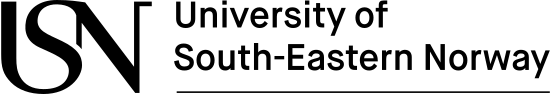
\includegraphics[width=\textwidth]{USN_logo_en}}
\institute{Faculty of Technology, Natural Sciences and Maritime Sciences}
%% use the following lines instead if you want the Norwegian logo and faculty
%\logo{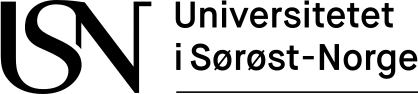
\includegraphics[width=\textwidth]{USN_logo}}
%\institute{Fakultet for teknologi, naturvitenskap og maritime fag}

\title{Title of Jane's Thesis}
\author[jane.doe@usn.no]{Jane Doe}
\date{\nth{28} May \the\year}
% If you don't want the date to appear that set it empty with:
% \date{}

\begin{document}

\begin{frame}{} % leave frame (sub)title empty
  \vskip1cm
  \begin{block}{\large Fontsizes}
    \centering {\tiny tiny}\par
    {\scriptsize scriptsize}\par
    {\footnotesize footnotesize}\par
    {\normalsize normalsize}\par
    {\large large}\par
    {\Large Large}\par
    {\LARGE LARGE}\par
    {\veryHuge VeryHuge}\par
    {\VeryHuge VeryHuge}\par
    {\VERYHuge VERYHuge}\par
  \end{block}
  \vskip1cm
  \begin{columns}[c]
    \begin{column}{0.45\linewidth}
      \begin{block}{Introduction}
        \begin{itemize}
        \item some items
        \item \alert{alert items}
        \item some items
        \item some items
        \end{itemize}
      \end{block}
      \vskip1cm
      \begin{block}{Theory}
        \begin{itemize}
        \item some items
        \item some items
        \item some items
        \item some items
        \end{itemize}
      \end{block}
      \vskip1cm
      \begin{block}{Set up}
        \begin{itemize}
        \item some items and $\alpha=\gamma, \sum_{i}$
        \item some items
        \item some items
        \item some items
        \end{itemize}
          $$\alpha=\gamma, \sum_{i}$$
      \end{block}
    \end{column}

    \begin{column}{0.5\linewidth}
      \begin{block}{Example}
        \begin{itemize}
        \item some items and $\alpha=\gamma, \sum_{i}$
        \item some items
        \item some items
        \item some items
        \end{itemize}
        $$\alpha=\gamma, \sum_{i}$$
      \end{block}
      \vskip1cm
      \begin{block}{Results}
        \begin{figure}[h]
          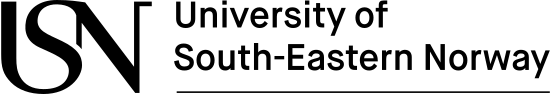
\includegraphics[width=.8\textwidth]{USN_logo_en}
          \caption{Example Figure}
        \end{figure}
      \end{block}
      \vskip1cm
      \begin{block}{Discussions}
        \begin{itemize}
        \item some items and $\alpha=\gamma, \sum_{i}$
        \item some items
        \item some items
        \item some items
        \end{itemize}
        $$\alpha=\gamma, \sum_{i}$$
      \end{block}
    \end{column}
  \end{columns}
\end{frame}

\end{document}
